\documentclass[11pt,letterpaper,twoside,english]{article}

\usepackage[margin=1.4in]{geometry} % controls the size of the margins

% Special symbols, etc.
\usepackage{amssymb,amsbsy,latexsym}
\usepackage{amsmath}
\usepackage{graphics, subfigure, float} 
\usepackage{cancel}
%\usepackage{todonotes}
% Encoding settings
\usepackage[latin1]{inputenc}
\usepackage[american]{babel}
\usepackage[T1]{fontenc} 
\usepackage{tikz}

\usepackage{titling} % allows posttitle command

% AMS Math packages

\usepackage{amscd,amsthm}

\usepackage{verbatim, comment} % can comment out text 
\usepackage{mdwlist} 

% Graphics
%\usepackage[dvips]{graphicx,epsfig,color}
%\usepackage{subfigure}
%\usepackage{pst-all}
%\usepackage{pstricks-add}
\usepackage{hyperref}  % can only be used with pdflatex - gives hyperlinks
\usepackage{bm} % bold math font
\usepackage{bbm}
\usepackage{todonotes}

\newtheoremstyle{theorem}{1em}{1em}{\slshape}{0pt}{\bfseries}{.}{ }{}
\theoremstyle{theorem}
\newtheorem{theorem}{Theorem}
\newtheorem*{theorem*}{Theorem}
\newtheorem{corollary}[theorem]{Corollary}
\newtheorem{proposition}[theorem]{Proposition}
\newtheorem{lemma}[theorem]{Lemma}
\newtheorem{claim}[theorem]{Claim}
\newtheorem{conjecture}[theorem]{Conjecture}
\newtheorem{definition}[theorem]{Definition}
\newtheorem*{claim*}{Claim}

\theoremstyle{remark}
\newtheorem{remark}{Remark}
\newtheorem*{remark*}{Remark}
\newtheorem{algorithm}{Algorithm}
\newtheorem*{question*}{Question}
\newtheorem{question}{Question}
\newtheorem{example}{Example}

\providecommand{\setN}{\mathbb{N}}
\providecommand{\setZ}{\mathbb{Z}}
\providecommand{\setQ}{\mathbb{Q}}
\providecommand{\setR}{\mathbb{R}}
\providecommand{\E}{\mathrm{E}}
\providecommand{\Pr}{\mathrm{Pr}}
\providecommand{\Var}{\mathrm{Var}}

\tikzset
{
    treenode/.style = {circle, draw=black, align=center, minimum size=1cm},
}

\makeatother

\title{18.821 Project 2} 

\author{Yajit Jain, Deepak Narayanan, Leon Zhang}

\begin{document}

\maketitle

\section{Introduction}

In this paper we will consider investigate pattern avoidance in permutations of finite sets of positive integers. 

\begin{definition}
Two finite sequences $a_1,\cdots a_k$ and $b_1,\cdots b_k$ have the same relative order if the $i^\text{th}$ largest entry of each unordered set $\{a_1,\cdots,a_n\}$ and $\{b_1,\cdots, b_n\}$ appears in the same position in $a_1\cdots a_k$ and $b_1\cdots b_k$ for each $1\le i\le k$. 
\end{definition}

\begin{definition}
A finite sequence of numbers $a_1a_2\cdots a_n$ avoids a sequence $b_1\cdots b_k$ with $n\ge k$ if no subsequence $a_{i_1}a_{i_2}\cdots a_{i_k}$ of $a_1a_2\cdots a_n$ has its terms in the same relative order as $b_1\cdots b_k$. 
\end{definition}

\begin{example}
The sequence 15432 avoids 123 while the sequence 13425 does not. The latter example fails because 134 appears in 15342 with the same relative order as 123. 
\end{example}


\begin{remark}
Let $S_n$ be the set of permutations of $\{1,\cdots, n\}$. There are two conventions commonly used to write elements of $S_n$. The first is $\emph{one-line}$ notation where permutations in $S_n$ are written explicitly, e.g. 43215 is a permutation of $\{1,2,3,4,5\}$ in $S_5$. 

The second is \emph{cycle notation}, where a cycle $(a_1\cdots a_n)\in S_n$ with $1\le a_i\le n$ acts on a sequence by sending $a_1\mapsto a_2$, $a_2\mapsto a_3$, $\cdots$, $a_n\mapsto a_1$. For example, the cycle $(14)(23)$ sends $12345$ to $43215$. Unless otherwise stated, we will refer to permutations in one-line notation. 
\end{remark}

\begin{definition} 
When $n\ge k$, a permutation $\sigma\in S_n$ avoids a permutation $\pi\in S_k$ if $pi$ and $\sigma$ avoid each other when written as sequences in one-line notation. 
\end{definition}

\begin{definition}
For a permutation $\pi$, we write $s_n(\pi$ for the number of permutations in $S_n$ that avoid $\pi$. 
\end{definition}

In this paper we concern ourselves with the sequences $s_n(\pi)$ for various $\pi$. In section \ref{S3} we will consider sequence $s_n(\pi)$ for $\pi\in S_3$, and in section \ref{S4} we will consider sequence $s_n(\pi)$ for $\pi\in S_4$. In section \ref{Tn} we consider a variation on the avoidance problem that considers the problem of avoiding sequences in a subset $T_n$ of $S_n$. 

\subsection{Generating Trees}

Before continuing we introduce generating trees, a tool we can use to study pattern avoidance. The generating tree for the sequence $s_n(\pi)$ is the infinite tree whose vertices are elements of $S_n$ that avoid $\pi$. To construct the tree, we define the children of an arbitrary node. Let $\omega\in S_k$ be a node of the generating tree of $s_n(\pi)$. Then the children of $\omega$ are elements of $S_{k+1}$ that avoid $\pi$ and that can be obtained by inserting the integer $k+1$ between integers in $\omega$. Figure \ref{fig:M1} is an example of the generating tree of $s_n(312)$. 

\begin{figure}[h!]
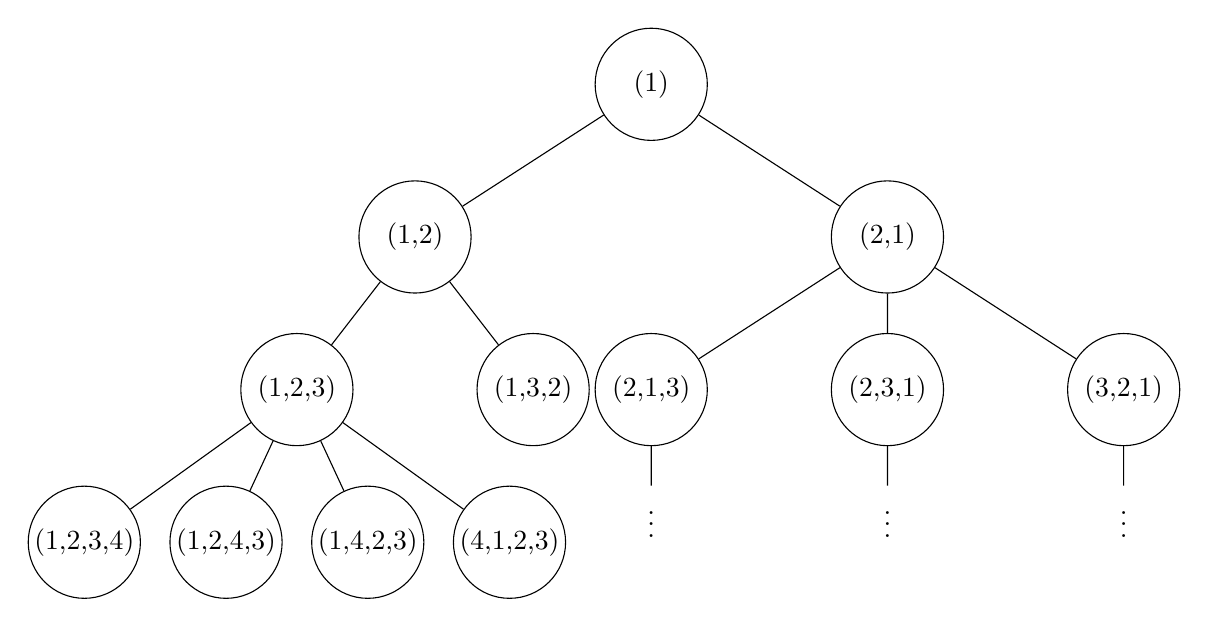
\begin{tikzpicture}[level distance=0.5cm, growth parent anchor={south}, nodes={anchor=north}]
\tikzstyle{hollow node}=[circle,draw,inner sep=0.1mm, text width=1.36cm,align=center]
\tikzstyle{level 1}=[sibling distance=6cm] 
\tikzstyle{level 2}=[sibling distance=3cm] 
\tikzstyle{level 3}=[sibling distance=1.8cm]
\tikzstyle{level 4}=[sibling distance=0.9cm]
\node [hollow node]{(1)}
	child {
		node[hollow node] {(1,2)}
		child{
			node[hollow node]{(1,2,3)}
			child{node[hollow node]{(1,2,3,4)}}
			child{node[hollow node]{(1,2,4,3)}}
			child{node[hollow node]{(1,4,2,3)}}
			child{node[hollow node]{(4,1,2,3)}}
		}
		child{
			node[hollow node]{(1,3,2)}
		}
	}
    	child {
		node[hollow node] {(2,1)}
    		child {
			node[hollow node] {(2,1,3)}
			child{node{\vdots}}
		}
      		child {
			node[hollow node] {(2,3,1)}
			child{node{\vdots}}
		}
		child {
			node[hollow node] {(3,2,1)}
			child{node{\vdots}}
		}
    	};

\end{tikzpicture}
\caption{Generating tree of the sequence $s_n(312)$} \label{fig:M1}
\end{figure}

\section{Terms in the sequence $s_n(312)$}
\label{S3}




We claim that the sequence of numbers $s_n(312)$ is in fact the sequence of Catalan numbers. We state this result formally as the following theorem,

\begin{theorem}
The total number of permutations of $\{1,2,3,...,n\}$ that avoid the order $312$ as a subsequence is $C_n$ where $C_n$ is the $n^{th}$ Catalan number.
\end{theorem}

Before proving the theorem, we state and prove the following lemma, that will be used in our proof of the theorem.
\begin{lemma}
All permutations of $\{1,2,\dots,k,k+1\}$ ending in $i$ that avoid the order $312$ as a sub-sequence must be of the form,
$$\pi_1 \pi_2 i$$
where $\pi_1$ is a permutation of $\{1,2,\ldots,(i-1)\}$ that avoids the order $312$ as a sub-sequence and $\pi_2$ is a permutation of $\{(i+1),\ldots,(k+1)\}$ that avoids the order $312$ as a sub-sequence.
\end{lemma}

\begin{proof}
It is clear that any subsequences of the permutation $\pi = \pi_1 \pi_2 i$ must avoid $312$ if the entire permutation $\pi$ is to avoid $312$ as well; this implies that the permutations $\pi_1$ and $\pi_2$ must avoid $312$ as well.

We proceed with a proof by contradiction.

Before proceeding, we define the sets $A$ and $B$ to be $\{1,2,\ldots,(i-1)\}$ and $\{(i+1),(i+2),\ldots,(k+1)\}$ respectively. For the sake of contradiction, let us assume that there exists some permutation $\pi$ of $\{1,2,...,k,k+1\}$ that ends with value $i$ such that some integer $x < i$ (that is, $x \in A$) is to the right of some integer $y > i$ ($y \in B$). Clearly, this permutation is not of the form described above. It is also easy to see that $\pi$ does \emph{not} avoid the order $312$ since the triple $(y, x, i)$ satisfies the condition $y > x > i$ and is in the order $312$.

From this we conclude that only permutations of the form described above can avoid $312$.

\end{proof}

With this lemma proven, we move on to the proof of our theorem.

\begin{proof}
The inductive hypothesis holds for our base case of $\{1\}$, since the only permutation of $\{1\}$ trivially avoids $312$.

Now, we need to prove the inductive case. Let us first assume that for all $i$ from $1$ to $k$, the number of permutations of $\{1,2,...,i\}$ that avoid the order $312$ as a subsequence is $C_i$.

Now, we want to prove the inductive hypothesis for $\{1,2,...,k,k+1\}$ as well, that is the number of permutations of $\{1,2,...,k,k+1\}$ that avoid the order $312$ as a subsequence is $C_{k+1}$.

We count the number of permutations of $\{1,2,...,k,k+1\}$ that avoid $312$ by enumerating through all possible values of the last term of a valid permutation.
If the last term of the permutation is $i$ (where $i \in \{1,2,...,k,k+1\}$), then let us define the subsets $A$ and $B$ of the  set $\{1,2,...,k+1\} \setminus \{i\}$ as the set of integers less than $i$ and the set of integers greater than $i$ respectively. It is clear from the definition of $A$ and $B$ that $A$ and $B$ are disjoint from each other.

Now, from the above lemma, we know that all permutations of $\{1,2,...,k,k+1\}$ ending in $i$ that avoid $312$ must be of the form,

$$\pi = \pi_1 \pi_2 i$$

where $\pi_1$ is a permutation of $A$ that avoids the order $312$ as a sub-sequence and $\pi_2$ is a permutation of $B$ that avoids the order $312$ as a sub-sequence. It is clear that the above permutation contains all integers between $1$ and $k+1$, from the definitions of the subsets $A$ and $B$, which implies that $\pi_1\pi_2i$ is permutation of the set $\{1,2,...,k,k+1\}$.

Now, the total number of permutations $\pi$ is,
$$n_{\pi_1} \cdot n_{\pi_2} = C_{i-1} \cdot C_{k-i+1}$$
since the total number of valid permuations $\pi_1$ is simply going to be $C_{i-1}$ (total number of valid permutations of length $i-1$ that avoid the order $312$ as a sub-sequence is $C_{i-1}$; similarly $n_{\pi_2} = C_{k-1+1}$)

Now, summing over all possible values of $i$, we see that the total number of permutations of $\{1,2,...,k+1\}$ that avoid $312$ is equal to,
$$\sum_{i=1}^{k+1} C_{i-1} \cdot C_{k-i+1} = \sum_{i=0}^k C_i \cdot C_{k-i}$$ which is in fact $C_{k+1}$, and we are done.

\end{proof}

\section{Conjectures on $s_n(\pi)$ for $\pi\in S_4$}
\label{S4}

\section{Avoidance of permutations of $T_n$}
\label{Tn}
We now impose further restrictions on the set of permutations $S_n$. This new set of permutations, $T_n$ is defined follows.

\begin{definition}
For even $n$, $T_n$ is defined as the set of all permutations $\sigma \in S_n$ for which $1,3,5,\ldots,2n-1$ appear in increasing order, and $2i$ always appears to the right of $2i-1$.
\end{definition}

Since $T_n$ is only defined for even $n$, henceforth we shall refer to $T_n$ as $T_{2m}$ where $m$ is any integer greater than or equal to $0$.

Given the above definition of $T_{2m}$, we prove the following result about the cardinality of $T_{2m}$.

\begin{theorem}
$|T_{2m}| = 1 \cdot 3 \cdot 5 \cdot \ldots \cdot (2m-1)$
\end{theorem}

\begin{proof}
Observe that since $1,3,5,\ldots,2m-1$ must appear in increasing order in $T_{2m}$, our problem is now reduced to determining the relative order of $2,4,6,\ldots,2m$ with respect to each other, as well as with respect to $1,3,5,\ldots,2m-1$.

Let us first try to insert $2m$ into the sequence $1,3,5,\ldots,2m-1$. Clearly, the way $T_{2m}$ is defined, $2m$ can be inserted into only $1$ slot, the one following $2m-1$. (Here we define a slot as a gap between two existing elements of the sequence, or the gap that follows the last element of the sequence or the gap that precedes the first element of the sequence)

Now, let us try to insert $(2m-2)$ into the sequence. $(2m-2)$ can be inserted into $3$ slots in the sequence -- the one between $2m-3$ and $2m-1$, the one between $2m-1$ and $2m$ or the one following $2m$.

Now, if we try to insert $(2m-4)$ into this incompletely formed sequence, we will see that there are $5$ possible locations into which this number can be inserted. Continuing this for all even numbers upto $2$, we observe that the total number of ways such a sequence can  be created is equal to $1 \cdot 3 \cdot 5 \cdot \ldots \cdot (2m-1)$, as desired.
\end{proof}

\end{document}